\documentclass{article}

\usepackage[english]{babel}

\usepackage[letterpaper,top=2cm,bottom=2cm,left=3cm,right=3cm,marginparwidth=1.75cm]{geometry}

\usepackage{amsmath}
\usepackage{graphicx}
\usepackage[colorlinks=true, allcolors=blue]{hyperref}

\title{How Urbanization Affected Land Surface Temperature in Santa Clara County between 2015 and 2025}
\author{Jessica Fung}

\begin{document}
\maketitle

\begin{abstract}
abstract
\end{abstract}

\section{Introduction}
Urbanization is the result of human society continuing to grow and expand in its surrounding environment, constructing on land that was once unoccupied by human beings. New developments affect the ecology of the location on which they are being built. Man-made architecture, such as skyscrapers, affects the way wind travels, for example. Black asphalt raises the surface temperature of where it is laid. By continuing to urbanize, many cities face challenges such as raising temperatures, a decline of natural wildlife, and shrinking zoning areas fit to be built on. In Santa Clara County, the largest county in the San Francisco Bay Area, surface temperatures have steadily risen over the decade due to constant expansion. 


\section{Urbanization of Santa Clara County, California}

\subsection{Vegetation changes}
Between figures 1 and 2, there are multiple areas in Santa Clara County that has seen a decrease in vegetation index within the last decade. The map consists of data from the months of June to September. 

The areas are the following:
\begin{itemize}
    \item Upper Diablo Range by Calaveras Reservoir
    \item San Jose Foothills and mountains east of San Jose, CA
\end{itemize}

However, there are a few areas that have seen an increase in vegetation index within the last decade. 

Those areas are the following:

\begin{itemize}
    \item Pacheco Pass, by Pacheco State Park
    \item Foothills southwest of Morgan Hill, CA
\end{itemize}

\begin{figure}[hbt!]
\centering
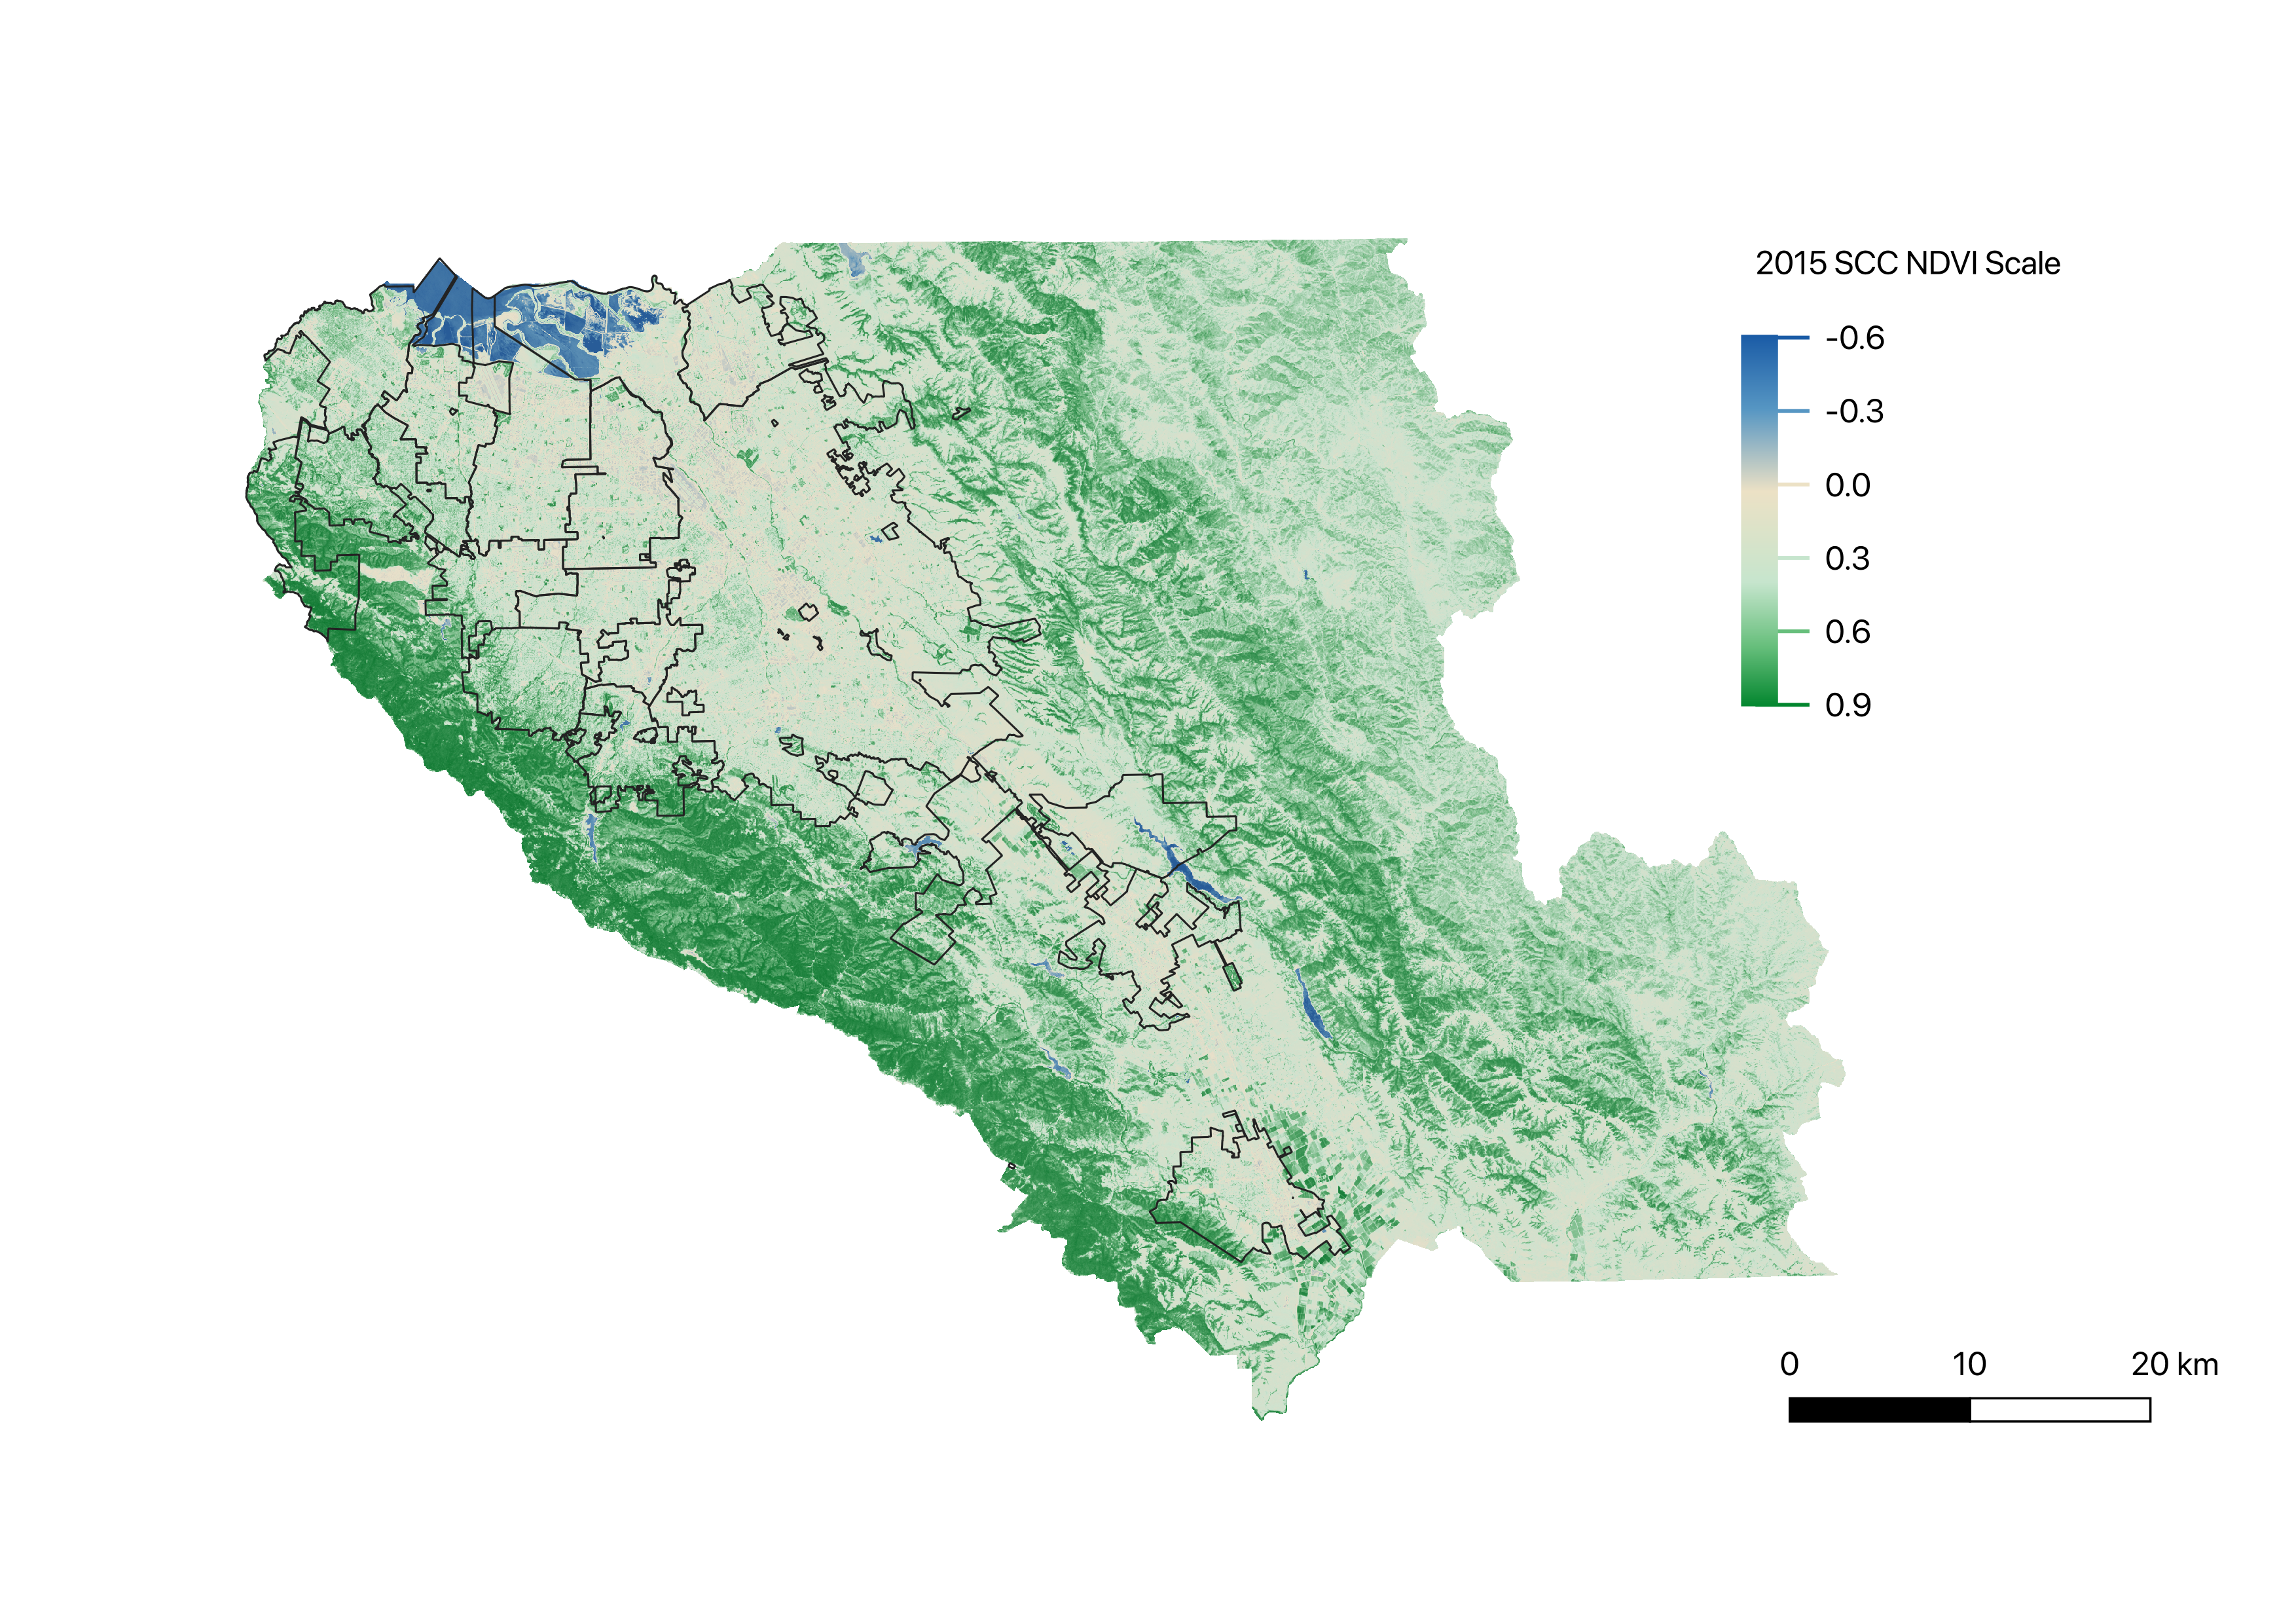
\includegraphics[width=0.8 \textwidth]{scc2015_ndvimap.png}
\caption{\label{fig:scc2015_ndvimap}An NDVI map of Santa Clara County in 2015 with city boundaries added.}
\end{figure}

\begin{figure}[hbt!]
\centering
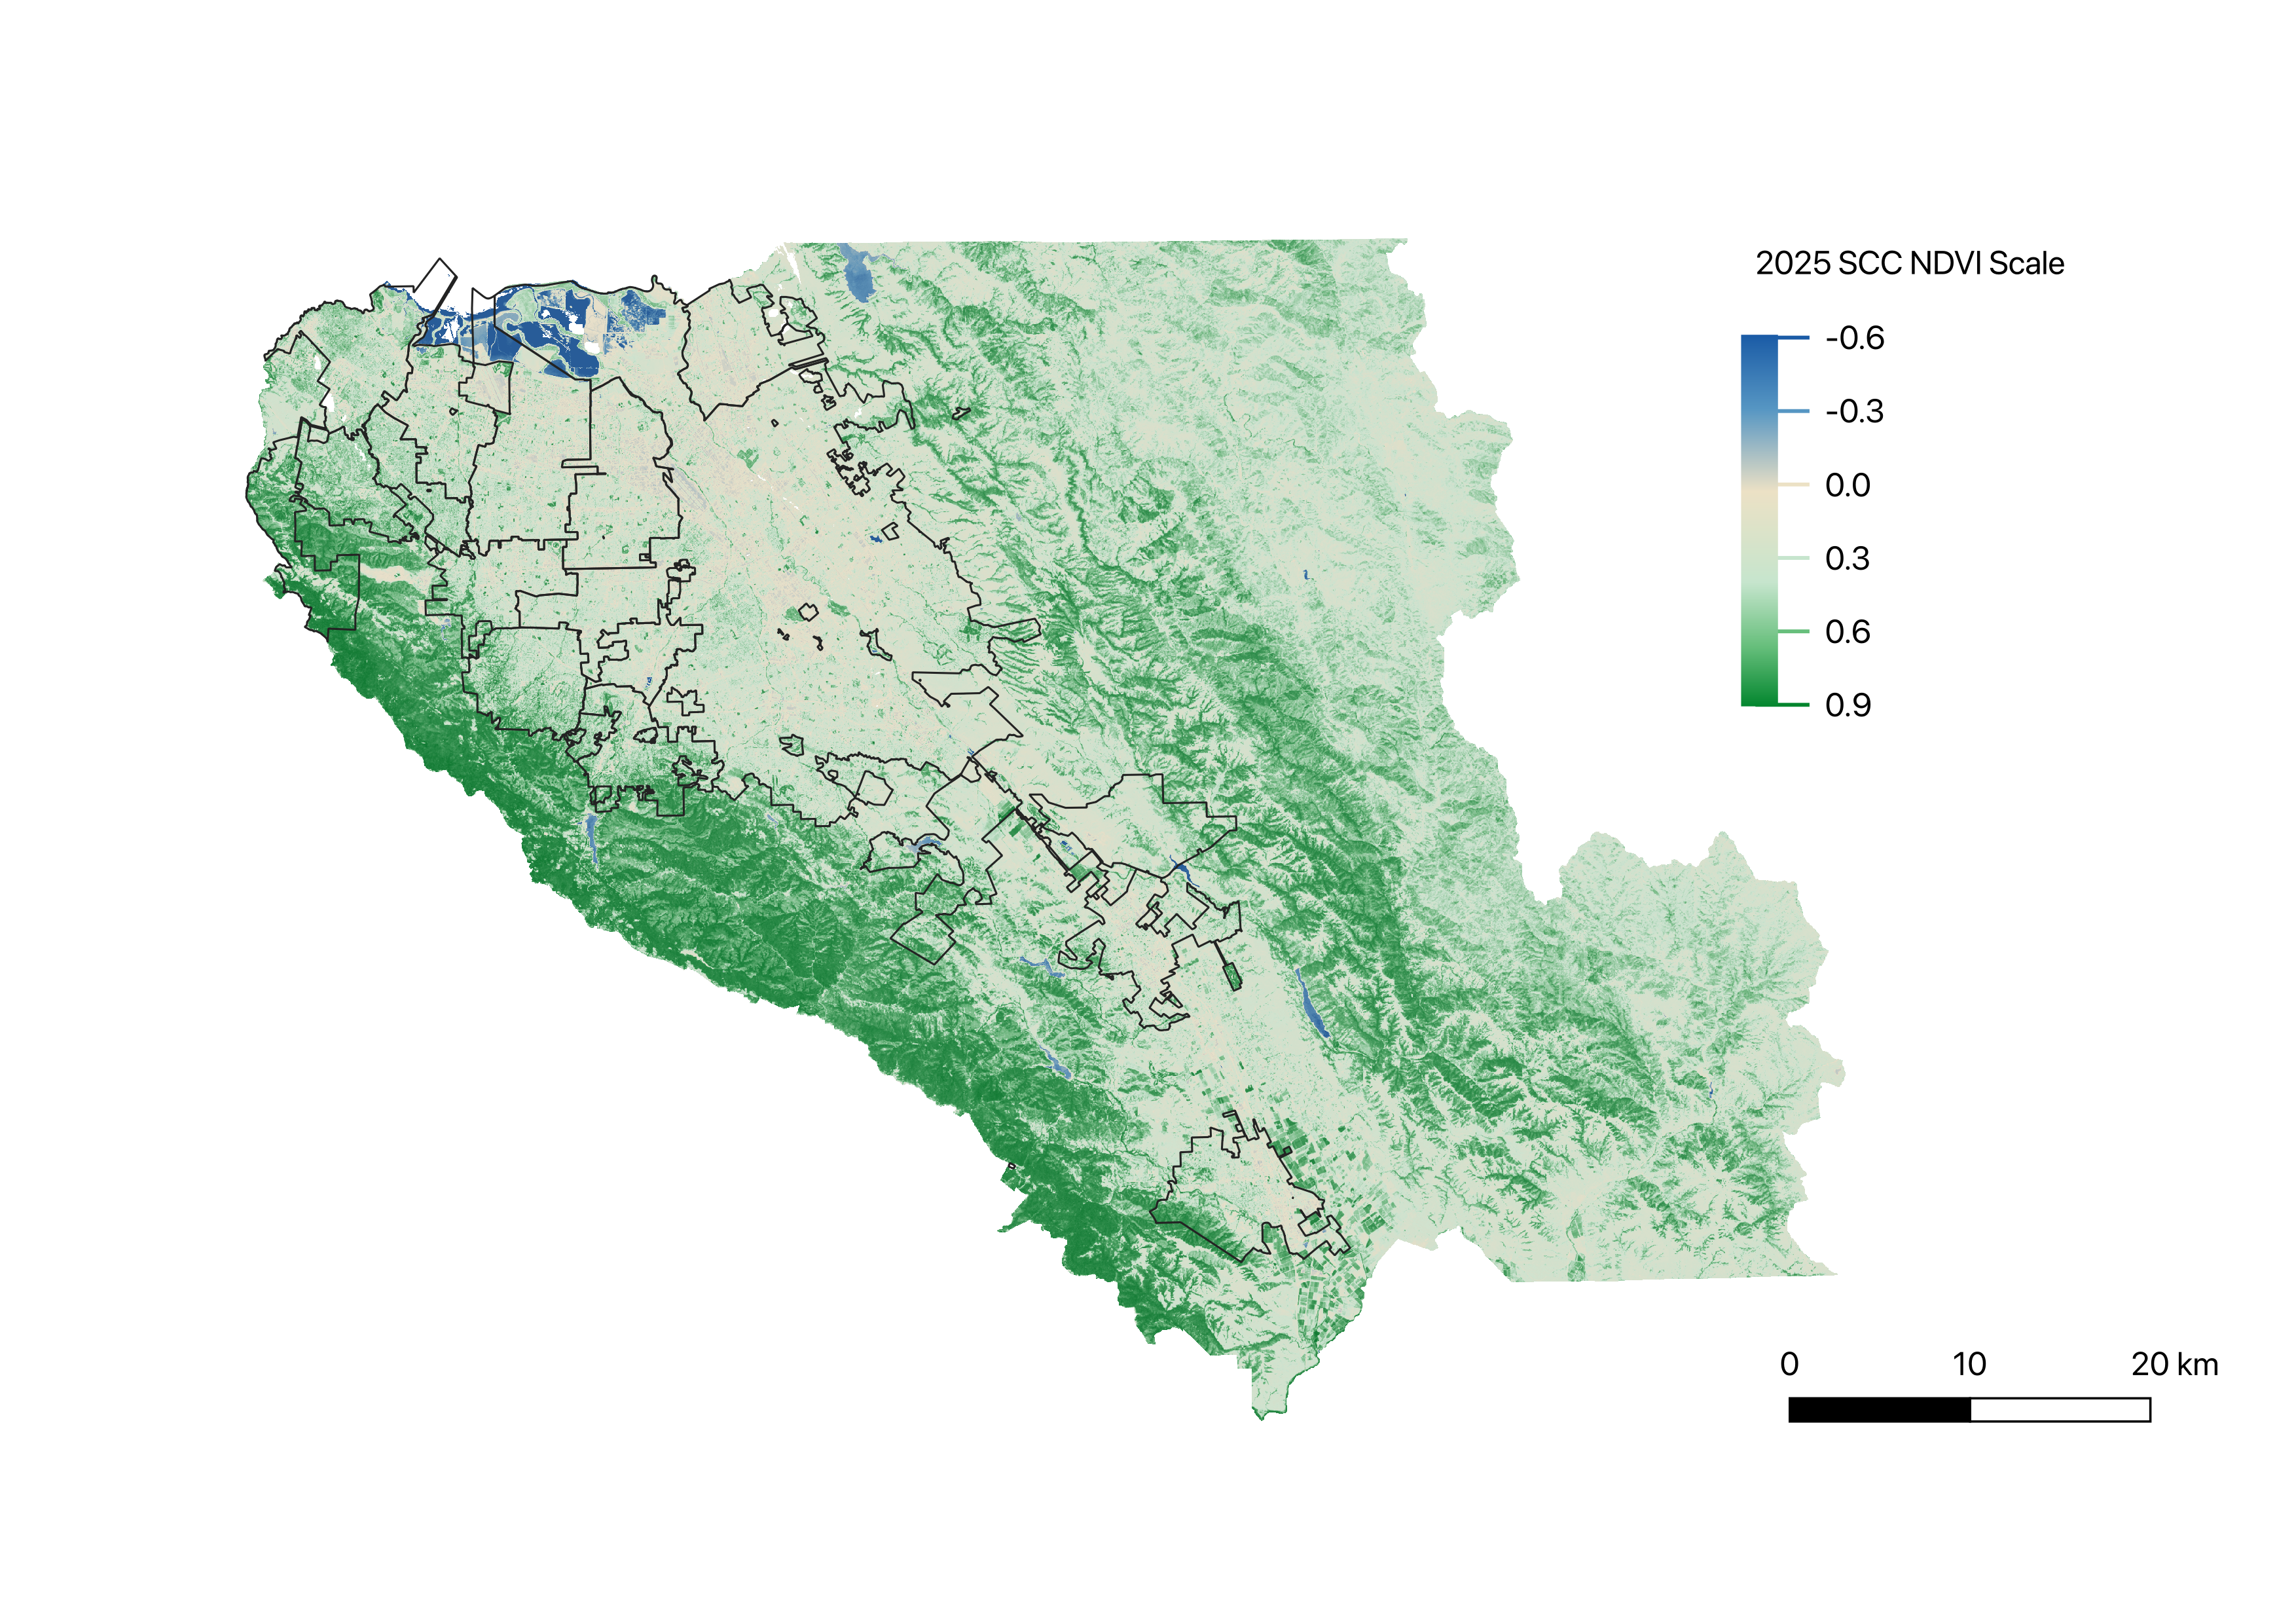
\includegraphics[width=0.8 \textwidth]{scc2025_ndvimap.png}
\caption{\label{fig:scc2025_ndvi}An NDVI map of Santa Clara County in 2025 with city boundaries added.}
\end{figure}

\subsection{Surface temperature changes}
Between figures 3 and 4, there are multiple areas in Santa Clara County that has seen an increase in surface temperature within the last decade. The map contains of data from the months of June to September. 

The areas are the following:
\begin{itemize}
    \item Diablo Range
    \item Santa Cruz mountains
    \item San Jose, CA
\end{itemize}

However, there are also areas that have seen a decrease in surface temperature within the last decade. 

Those areas are the following:
\begin{itemize}
    \item South Santa Cruz mountains close to Gilroy and Salinas
    \item Pacheco Pass, by Pacheco State Park
    \item Henry Coe State Park and the area south of the park
\end{itemize}

\begin{figure}[hbt!]
\centering
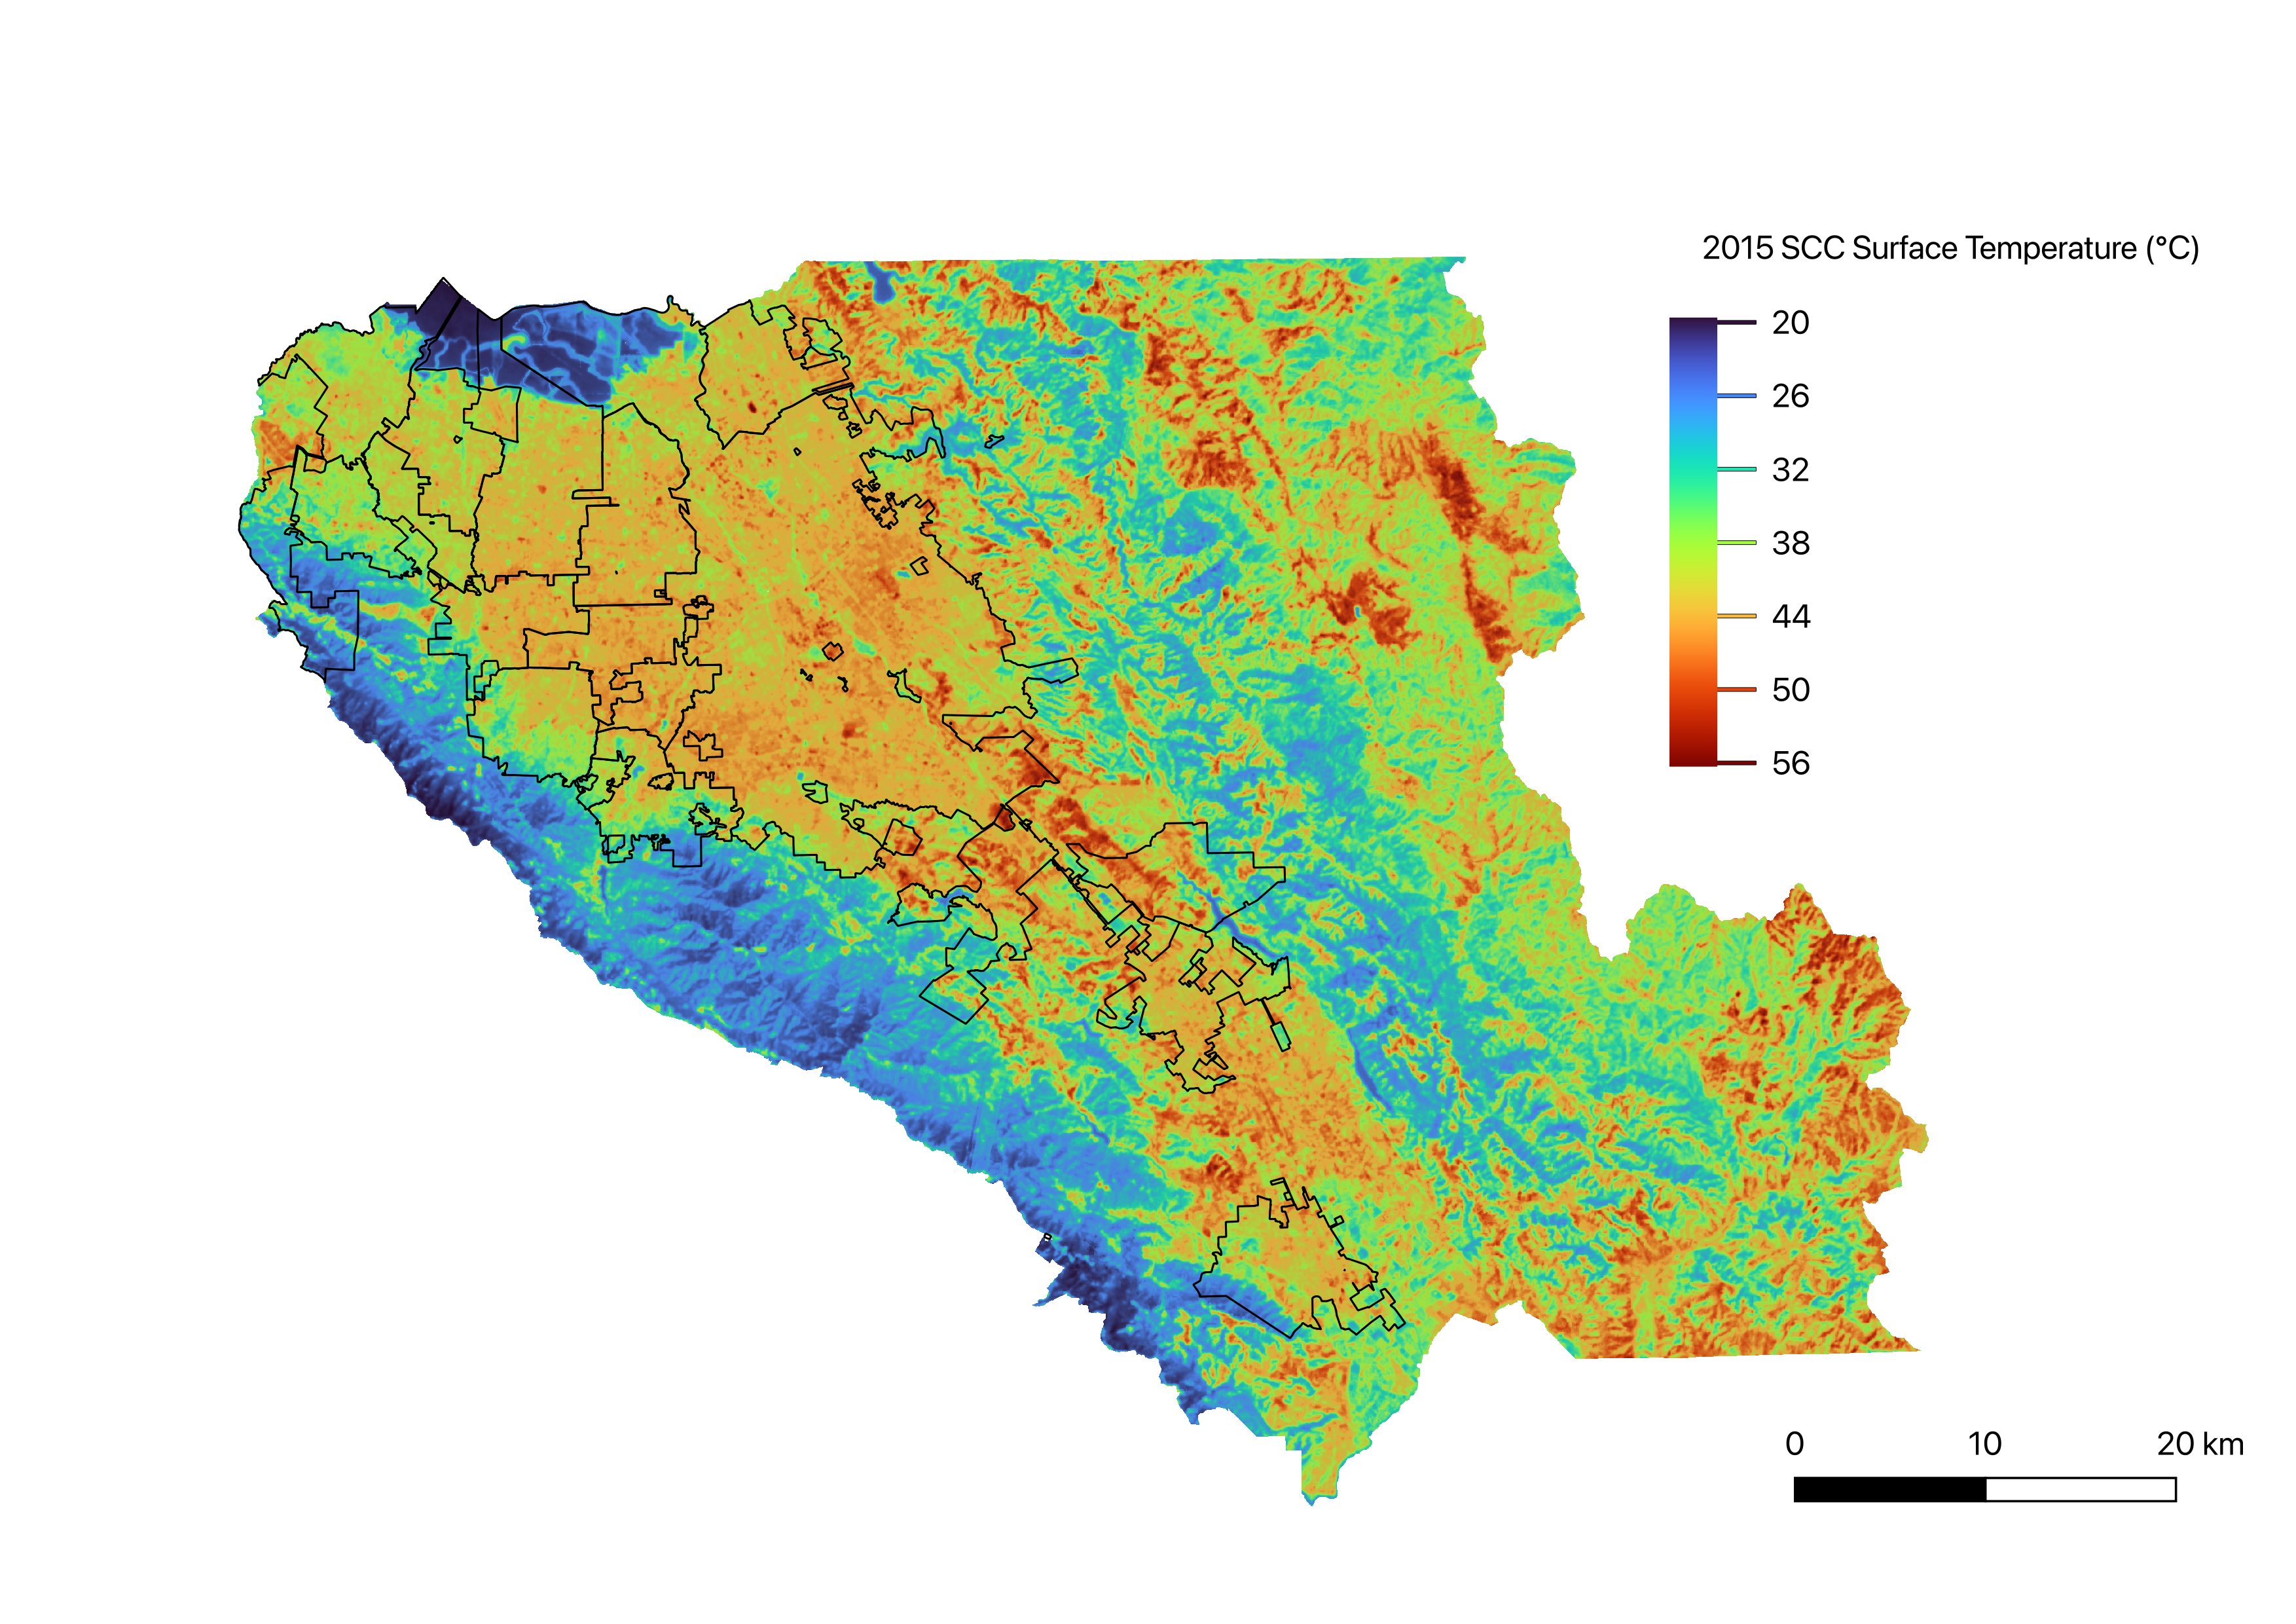
\includegraphics[width=0.8\textwidth]{scc2015_surftemp.png}
\caption{\label{fig:scc2015_surftemp}A surface temperature map of Santa Clara County in 2015 with city boundaries added.}
\end{figure}

\begin{figure}[hbt!]
\centering
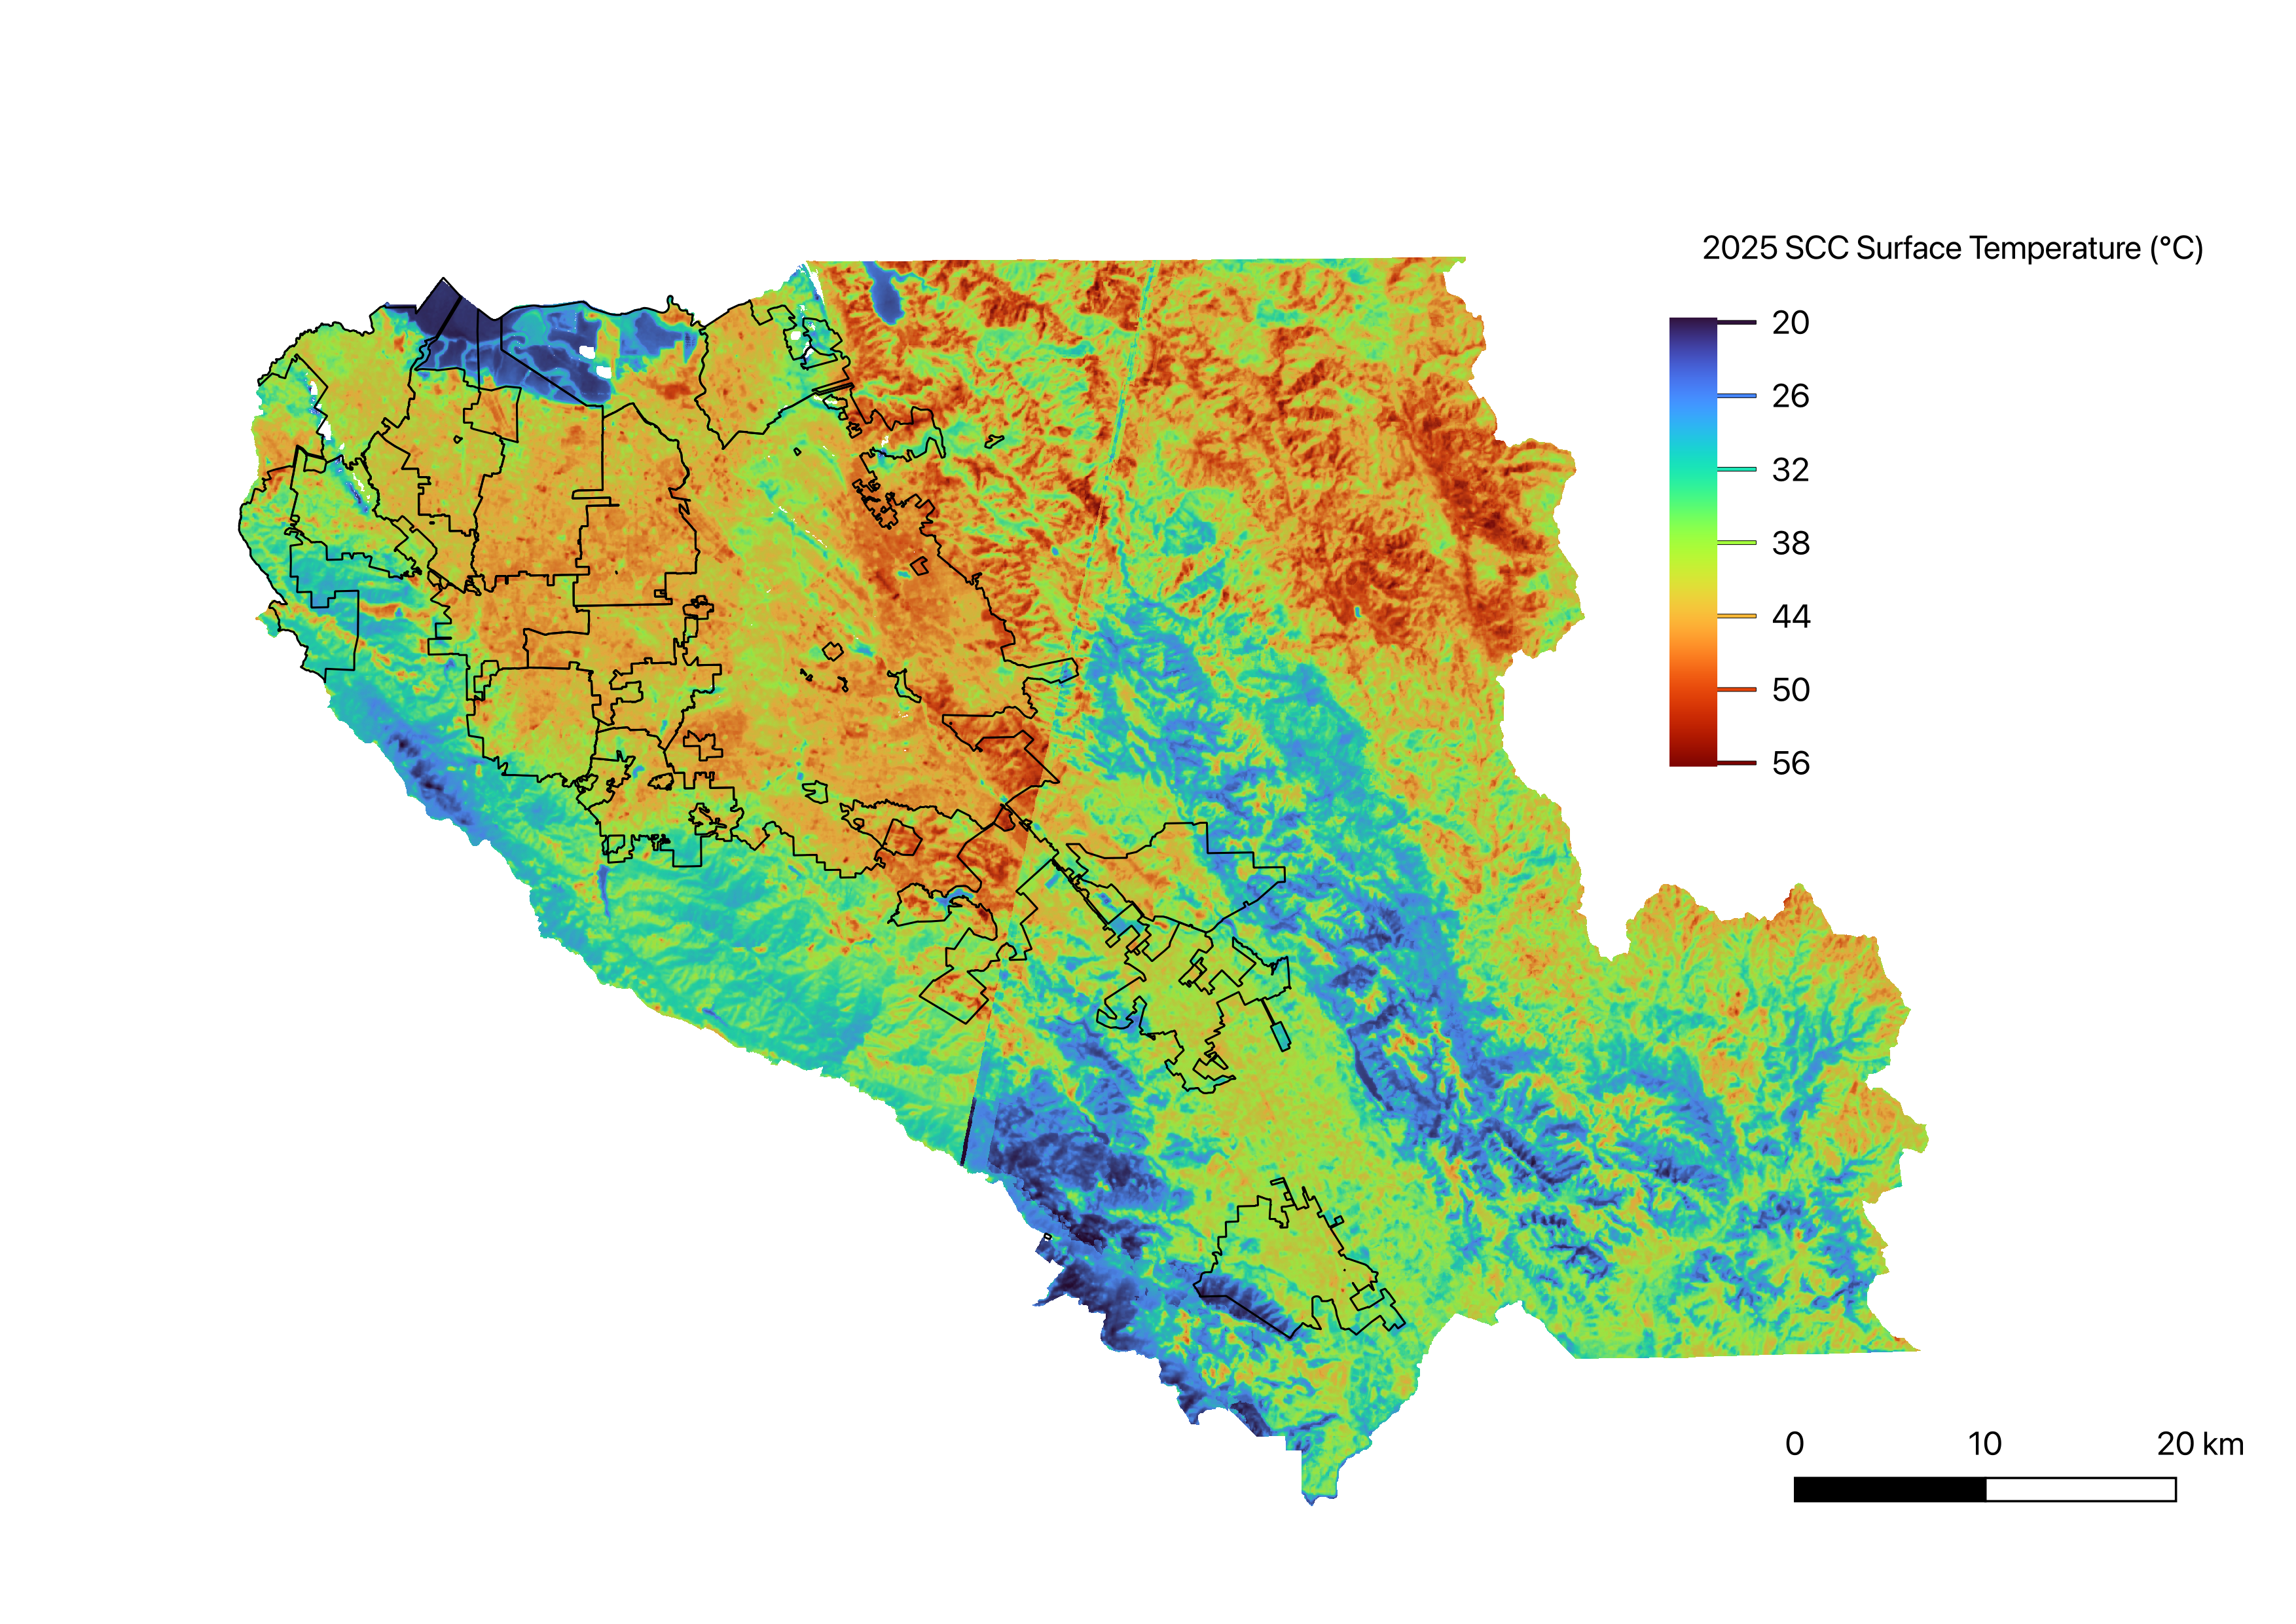
\includegraphics[width=0.8\textwidth]{2025surftemp_betterlegend.png}
\caption{\label{fig:2025surftemp_betterlegend}A surface temperature map of Santa Clara County in 2025 with city boundaries added.}
\end{figure}

It is noted that 2025 was considered a cold summer for the San Francisco Bay Area. Climate charts of San Jose, CA from 2015 and 2025 show a drastic difference in observed temperature between the two years, with 2015 showing higher observed temperatures during the summer months compared to 2025. 

In figure 5, it can be noted that San Jose had multiple days where the observed temperature was over 90 degrees Fahrenheit between the months of June to September, with majority of the peaks happening in September 2015.

In figure 6, it can be noted that San Jose had less days where the observed temperature was over 90 degrees Fahrenheit between the months of June to September. According to the figure, the highest observed temperature in July 2025 was in the high 80's. Similar to 2015, September had the most days with observed temperatures over 90 degrees. 

\begin{figure}[hbt!]
    \centering
    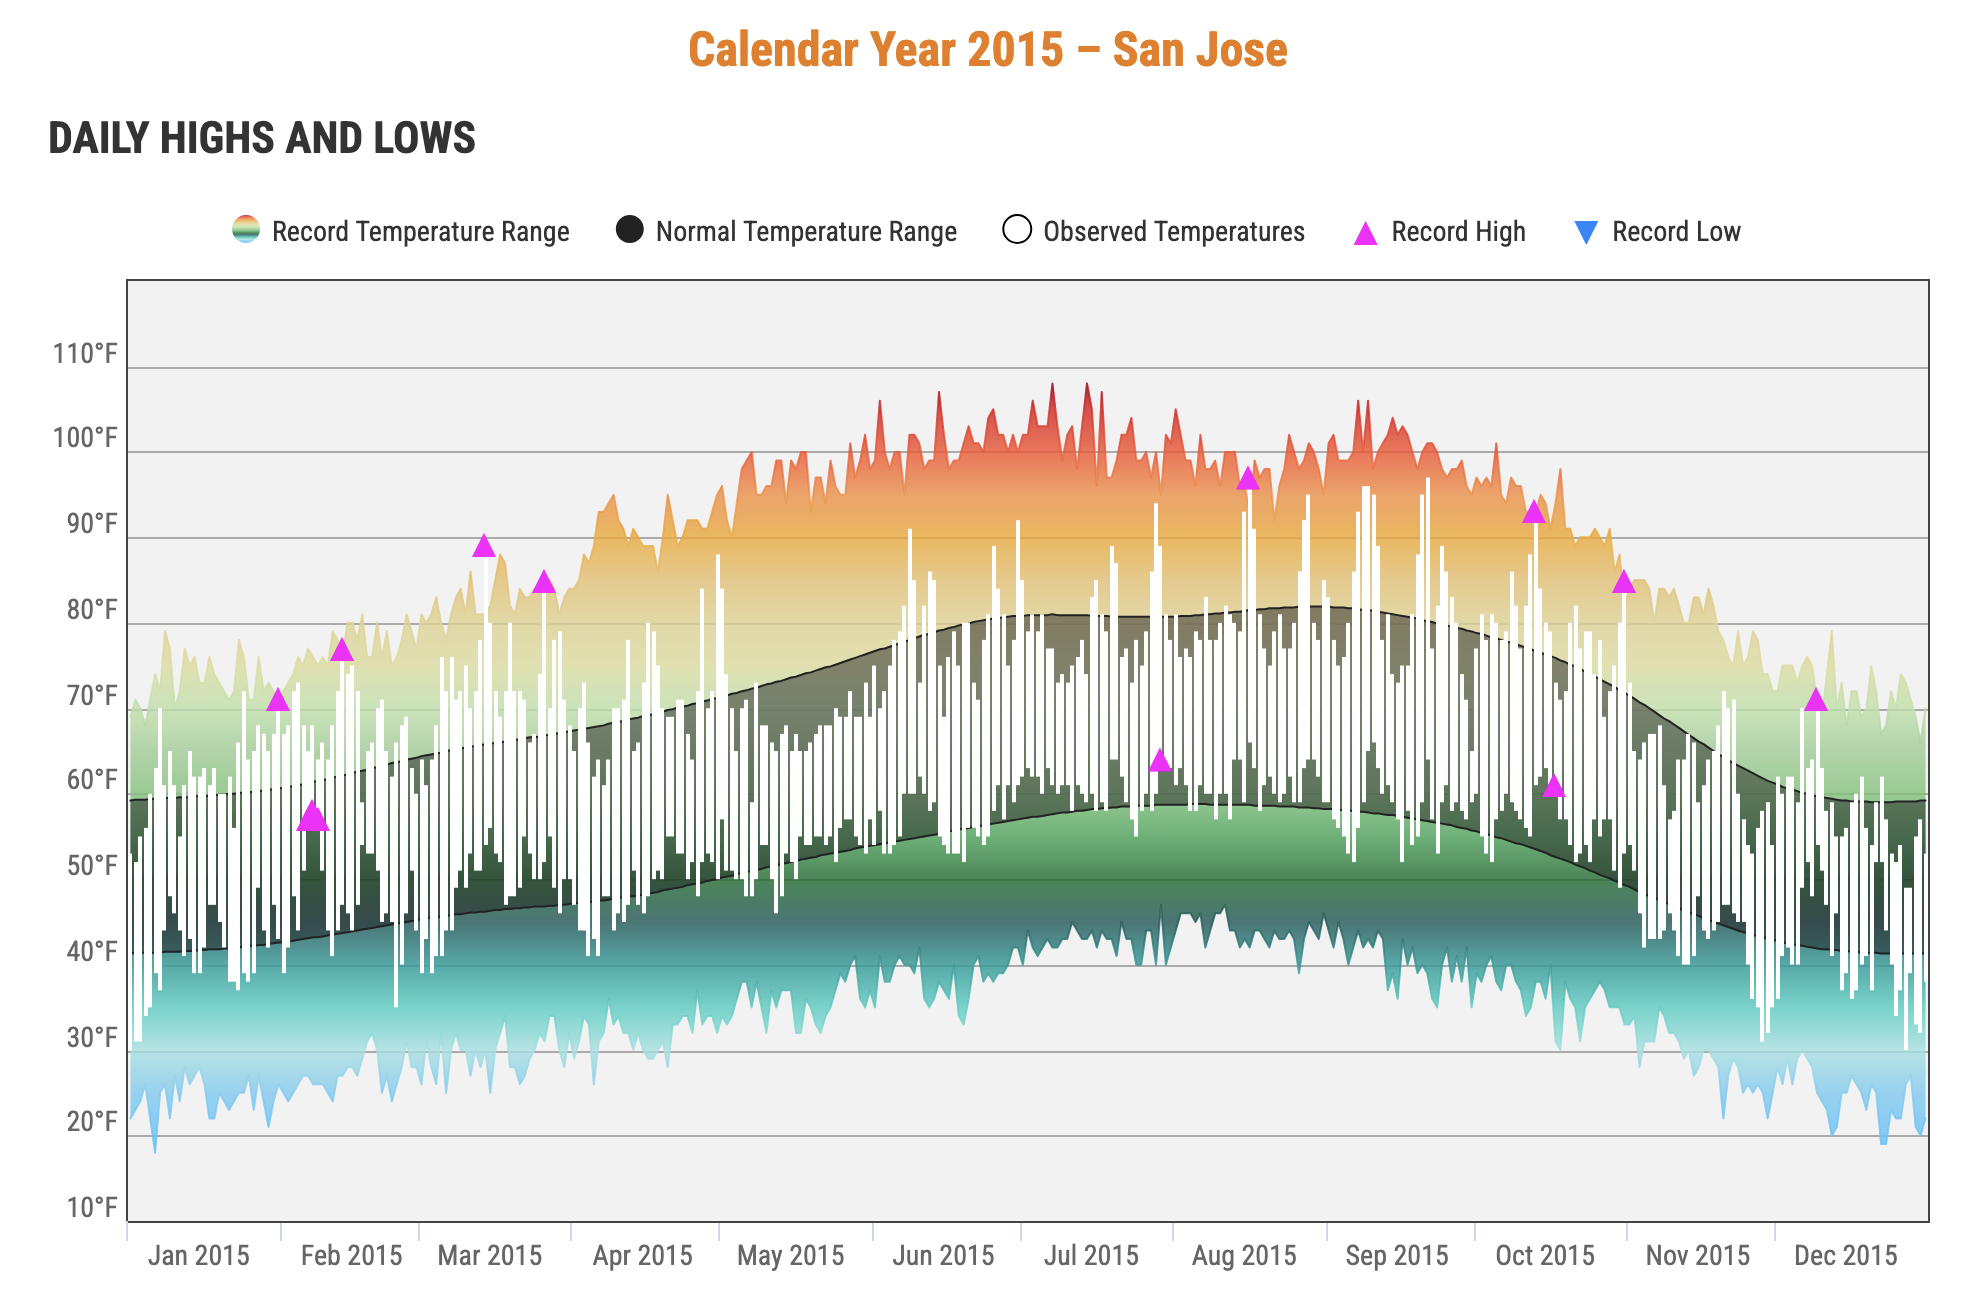
\includegraphics[width=0.8\textwidth]{sanjose2015yearlyclimate.png}
    \caption{\label{fig:sanjose2015yearlyclimate}NWS chart of San Jose climate in 2015}
    
\end{figure}

\begin{figure}[hbt!]
    \centering
    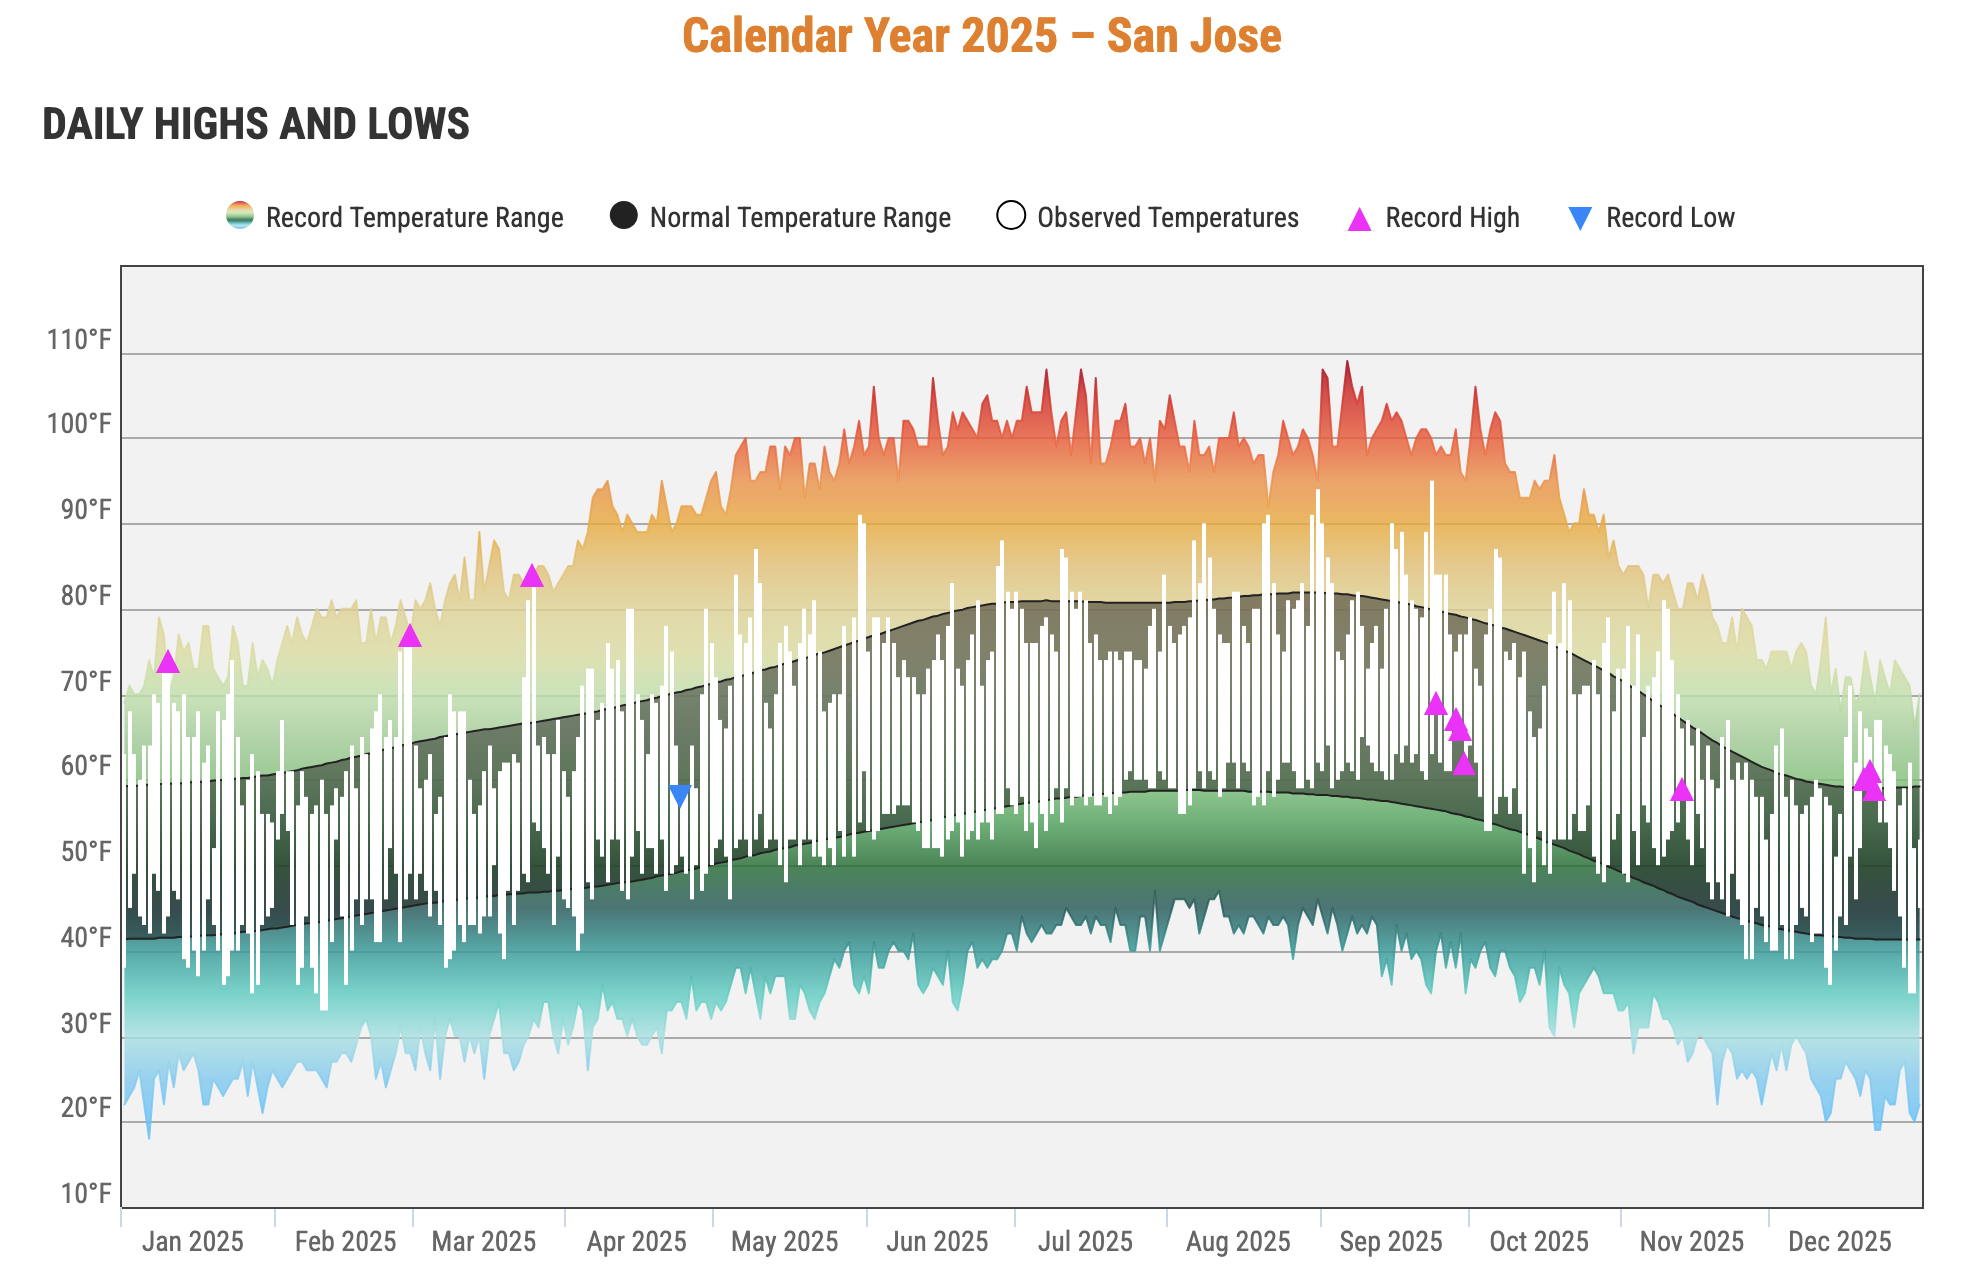
\includegraphics[width=0.8\textwidth]{sanjose2025yearlyclimate.png}
    \caption{\label{fig:sanjose2025yearlyclimate}NWS chart of San Jose climate in 2025}
    
\end{figure}

\bibliographystyle{alpha}
\bibliography{sample}


\end{document}